\begin{usecase}{Connect Calendar}
  \ucbasicinfo{Medium}{Regular}
  \ucshortdescription{This UC allows the user to connect their external calendars to our system.}
  \uctrigger{This UC is triggered when the user selects the option to connect an external calendar in the app.}
  \ucactors{User}{CalDAV}
  \ucpreconditions{User must be logged in}
  \ucrelationships{N/A}{N/A}{N/A}
  \ucinputsoutputs{
    \begin{itemize}
      \item \textbf{CalDAV login credentials and Name} (Source: User)
    \end{itemize}
  }{
    \begin{itemize}
      \item \textbf{Calendar data sync status} (Destination: System)
    \end{itemize}
  }
  \ucmainflow{
    \begin{enumerate}
      \item The user clicks the ``Connect Calendar'' option in the app.
        \ucinfo{The app asks the user to enter their CalDAV credentials along with a user provided name.}
      \item The system talks to the external calendar system via the credentials provided by the user.
        \ucinfo{The system adds the received calendar data to the database and a connection success status is shown to the user.}
      \item The system saves the CalDAV credentials securely in the database.
        \ucinfo{The credentials are encrypted before storing them.}
    \end{enumerate}
  }
  \ucalternateflows{
    \begin{enumerate}
      \item If the credentials are wrong or the request times out, the user can retry the request again.
    \end{enumerate}
  }
  \ucexceptions{
    \begin{itemize}
      \item Invalid credentials.
      \item Network issue with CalDAV server.
    \end{itemize}
  }
  \ucconclusion{The UC ends when the user has a successfully connected and synced external calendar with our system.}
  \ucpostconditions{The system has access to the user's external calendar, and events are synced and displayed for the user in the app..}
  \ucspecialrequirements{The system must handle multiple calendars efficiently.}
\end{usecase}

\begin{figure}[!h]
  \centering
  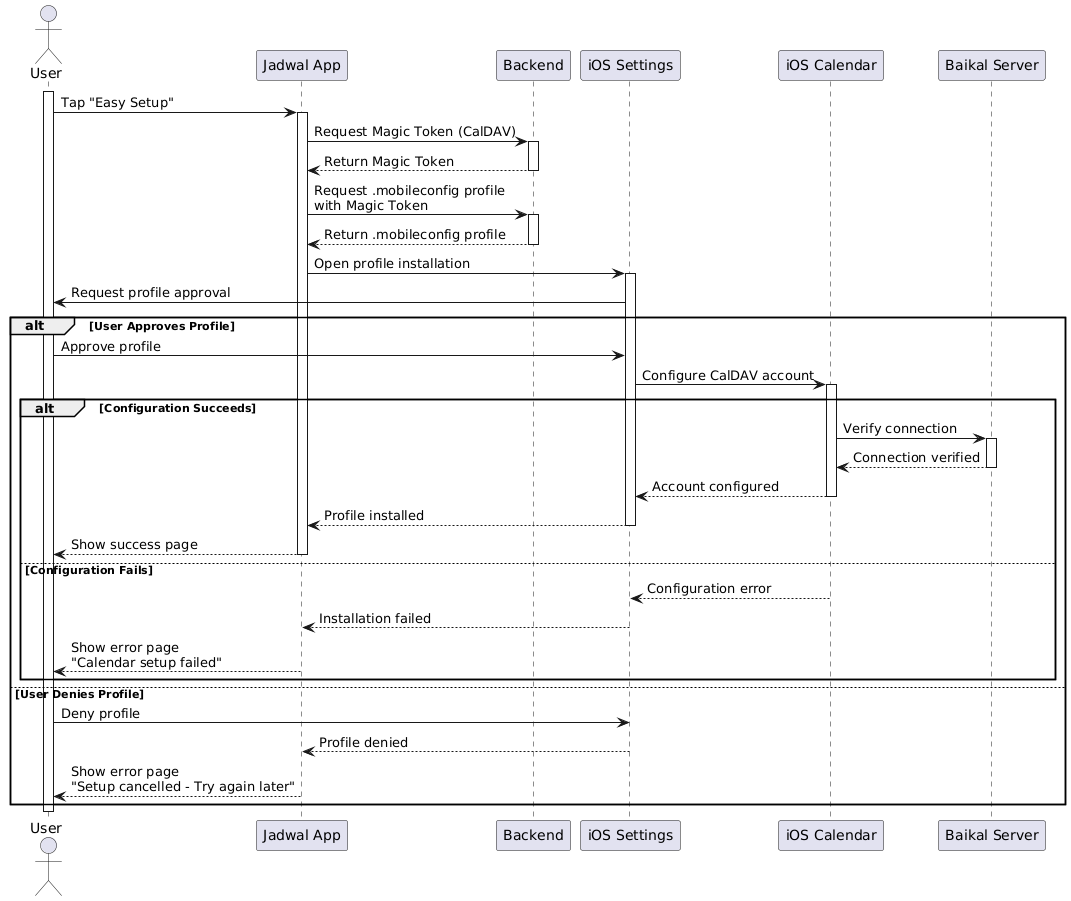
\includegraphics[width=\textwidth]{images/docs/diagrams/sequence-diagrams/all-sequence-diagrams/Connect Calendar.png}
  \caption{Connect Calendar Sequence Diagram}
  \label{fig:seq/connect-calendar}
\end{figure}